\documentclass[aspectratio=169]{beamer}

\usetheme{default}  % You can choose any other theme you prefer

\title{01 - Algoritmos}
\author{Mateus Oliveira de Figueiredo}
\date{\today}

\usepackage{tikz}
\usepackage{multicol}
\usepackage{algorithm}
\usepackage{algpseudocode}

\begin{document}

\begin{frame}
\titlepage
\end{frame}

\begin{frame}
\frametitle{Problema a ser resolvido}

\begin{overprint}
\onslide<1->{
  \begin{block}{Problema}
    Dado um polígono e um ponto P, determinar se P está dentro ou fora do polígono.
  \end{block}
}
\onslide<2>{
  \begin{block}{Teorema de Jordan}
    Seja C uma curva simples e fechada. O complementar de C possui duas componentes conexas, uma limitada e outra ilimitada. 
  \end{block}

  % add two columns to the slide
  \begin{columns}
    \column{0.5\textwidth}
    \begin{center}
      \begin{figure}
        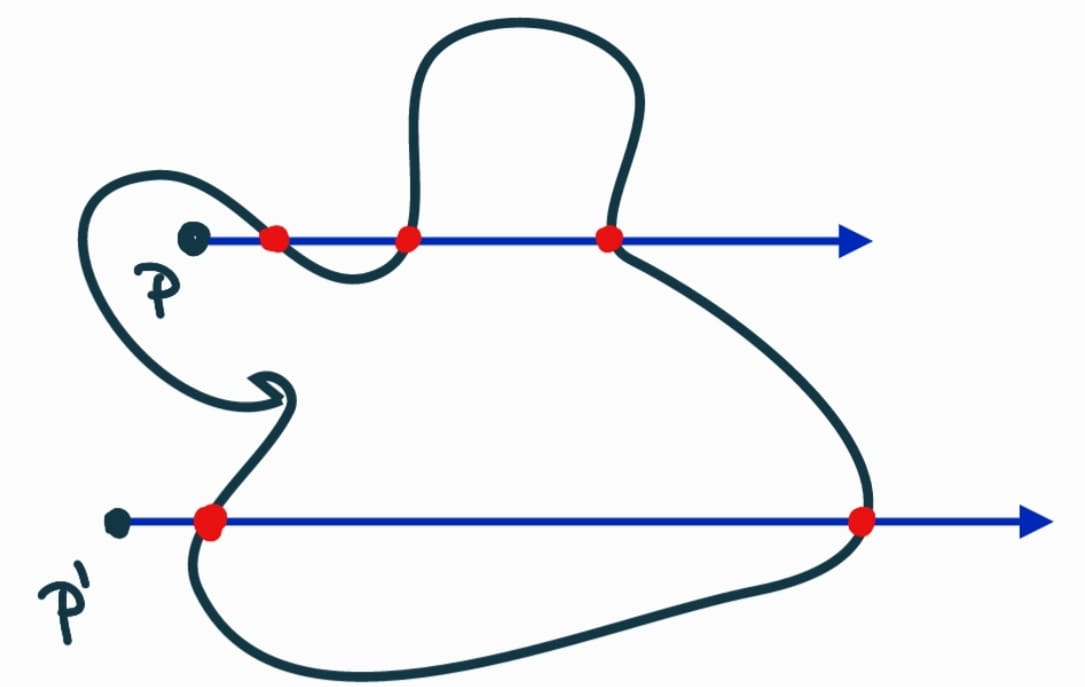
\includegraphics[width=0.8\textwidth]{figures/CurvaJordan.jpeg}
      \end{figure}
    \end{center}

    \column{0.5\textwidth}
    \begin{center}
      \begin{figure}
      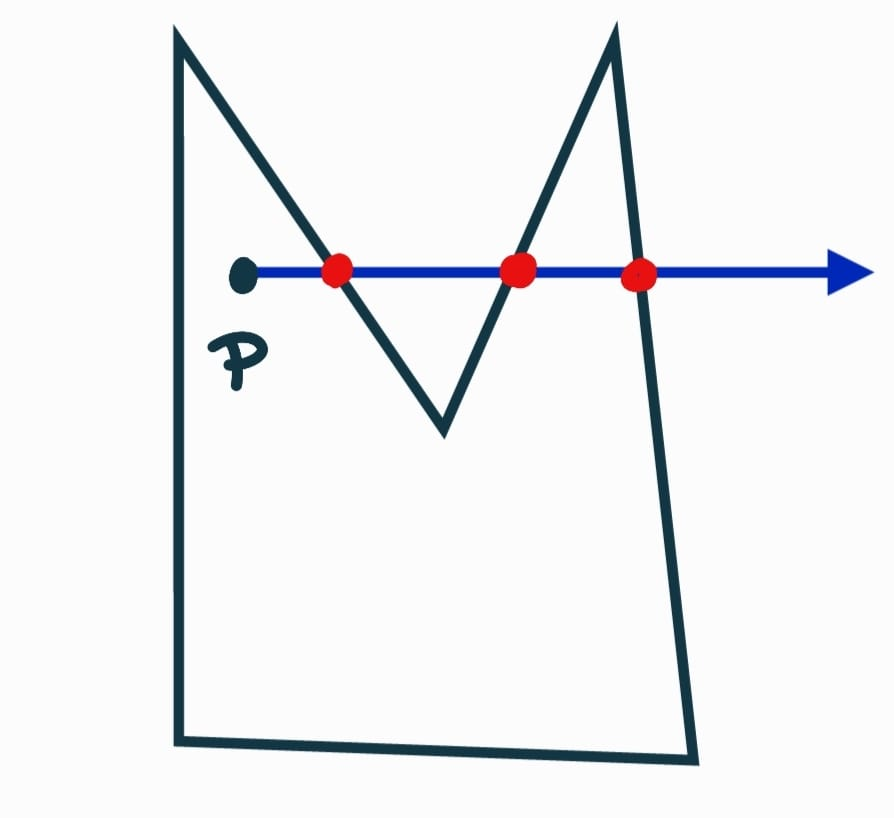
\includegraphics[width=0.6\textwidth]{figures/PolJordan.jpeg}
      \end{figure}
    \end{center}
}
\end{columns}

\end{overprint}

\end{frame}

\begin{frame}
\frametitle{Algoritmo de Interseção}
\begin{center}

\begin{columns}
  \column{0.5\textwidth}
  \begin{center}
    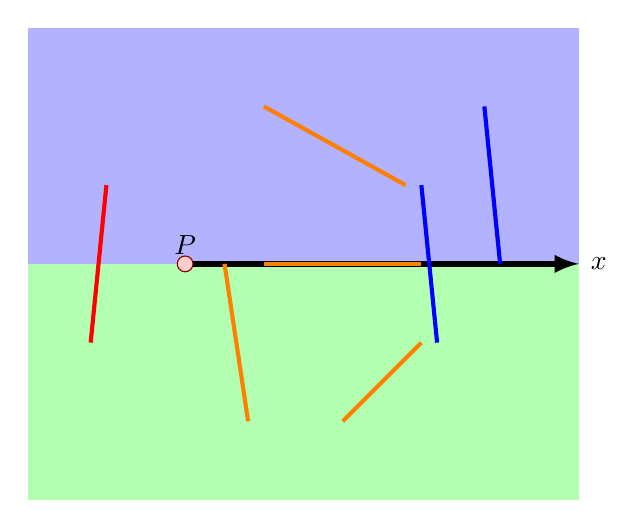
\begin{tikzpicture}
      % Upper Part
      \fill [blue!30] (-2,0) rectangle (5,3) node[midway] (omega_up) {$\Omega_{\text{up}}$};
      % Lower Part
      \fill [green!30] (-2,0) rectangle (5,-3) node[midway] (omega_down) {$\Omega_{\text{down}}$};
      % Axis
      \draw[-latex, line width=2pt, black] (0,0) -- (5,0) node[right] {$x$};
      % Point
      \filldraw[fill=red!20!white, draw=red!50!black] (0,0) circle (0.1) node[above] {$P$};

      % Segment
      \draw [orange, line width=1.5pt] (1, 2) -- (2.8, 1); 
      \draw [orange, line width=1.5pt] (2, -2) -- (3, -1); 
      \onslide<3-> {
        \draw [orange, line width=1.5pt] (1, 0) -- (3, 0); 
        \draw [orange, line width=1.5pt] (0.5, 0) -- (0.8, -2); 
      }
      \onslide<6-> {
        \draw [blue, line width=1.5pt] (3, 1) -- (3.2, -1);
        \draw [blue, line width=1.5pt] (4.0, 0) -- (3.8, 2);
      }
      
      \onslide<7->{
        \draw [red, line width=1.5pt] (-1, 1) -- (-1.2, -1);
      }
    \end{tikzpicture}
  \end{center}
  \column{0.5\textwidth}
  \begin{center} 
    \begin{overprint}
      \begin{algorithmic}
        \onslide<2->{
        \If{$(y_a > y_p \text{ and } y_b > y_p)$ or $(y_a \leq y_p \text{ and } y_b \leq y_p)$}
          \State \Return $\textcolor{orange}{false}$
        \EndIf
        }
        \onslide<4->{
        \State ${x_i} \gets {x_a} + \frac{{y_p - {y_a}}}{{y_b - {y_a}}}\left( {{x_b} - {x_a}} \right)$
        }
        \onslide<5->{
          \If{$x_i > x_p$}
            \State \Return $\textcolor{blue}{true}$
          \Else
            \State \Return $\textcolor{red}{false}$
          \EndIf
        }
        \end{algorithmic}
    \end{overprint}
  \end{center}
\end{columns}

\end{center}

\end{frame}

\begin{frame}{Exemplo 01}
  \begin{center}
    \begin{figure}
      \begin{overprint}
        \onslide<1>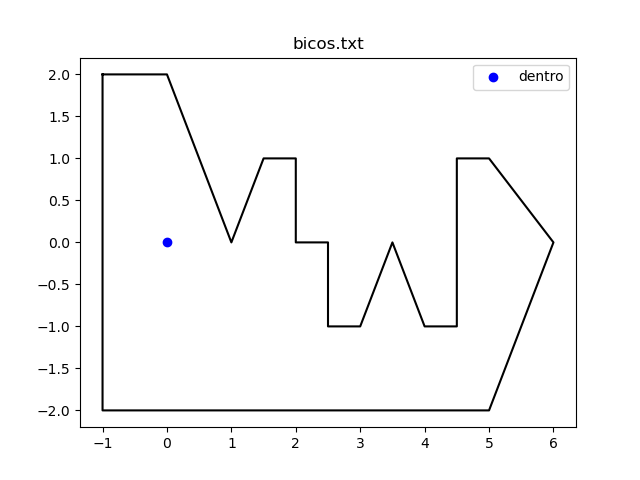
\includegraphics[width=0.8\textwidth]{figures/bicos.png}
        \onslide<2>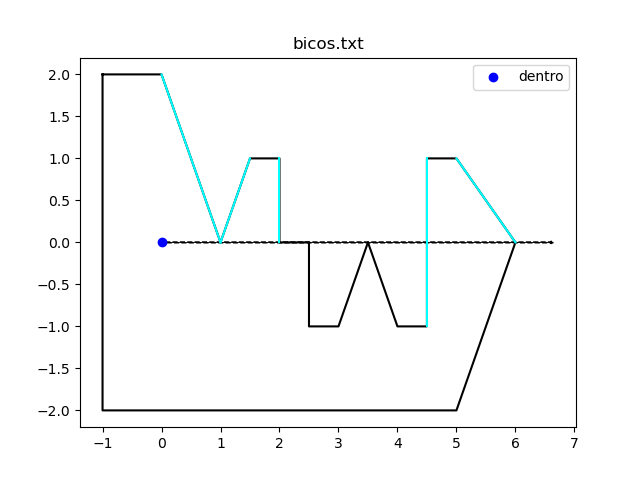
\includegraphics[width=0.8\textwidth]{figures/bicos_marcados.png}
        \onslide<3>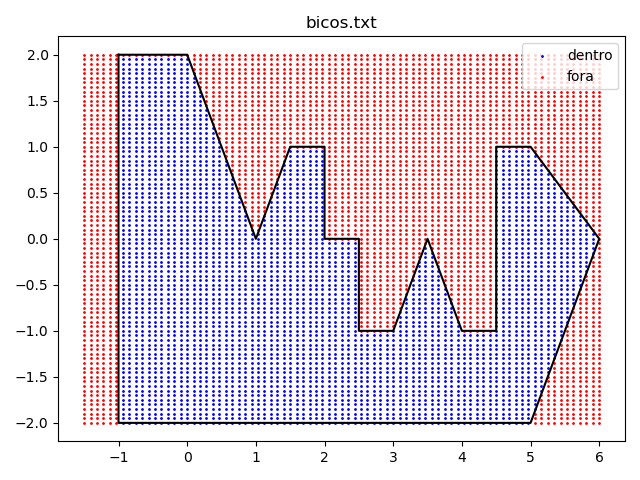
\includegraphics[width=0.8\textwidth]{figures/bicos_grid.png}
      \end{overprint}
    \end{figure}
  \end{center}
\end{frame}

\begin{frame}{Polígonos Simples}
  % add three columns
  \begin{columns}
    \column{0.33\textwidth}
    \begin{center}
      \begin{figure}
        \begin{overprint}
        \onslide<1>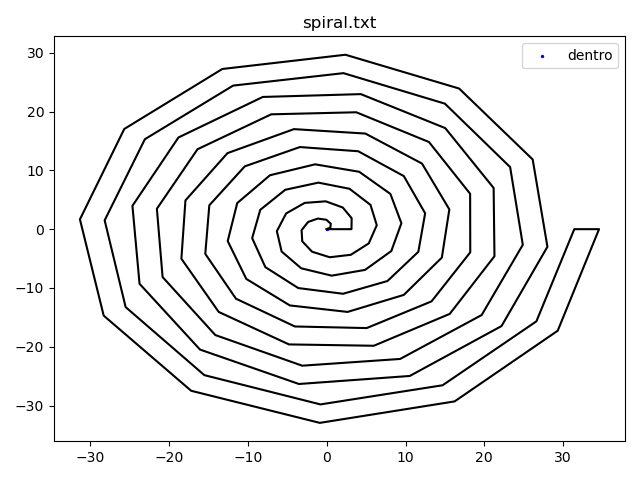
\includegraphics[width=1.0\textwidth]{figures/spiral.png}
        \onslide<2>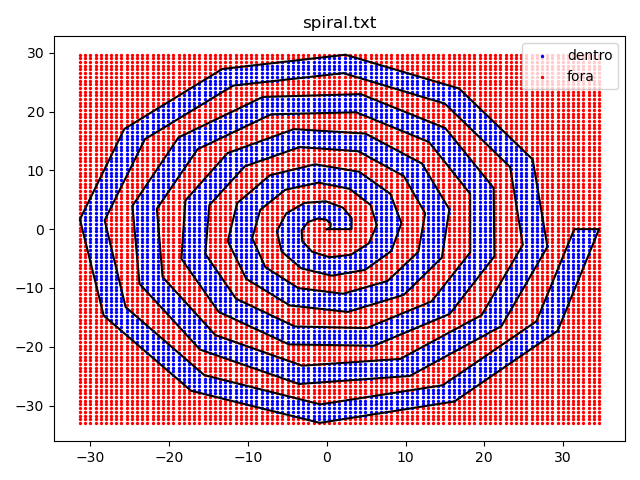
\includegraphics[width=1.0\textwidth]{figures/spiral_grid.png}
        \end{overprint}
      \end{figure}
    \end{center}
    \column{0.33\textwidth}
    \begin{center}
      \begin{figure}
        \begin{overprint}
        \onslide<1>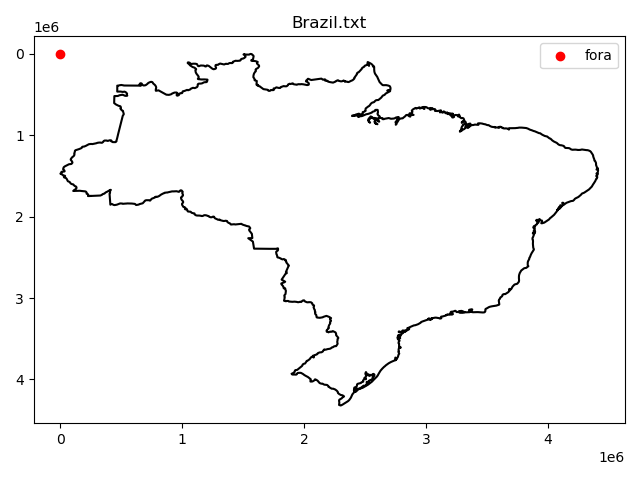
\includegraphics[width=1.0\textwidth]{figures/Brazil.png}
        \onslide<2>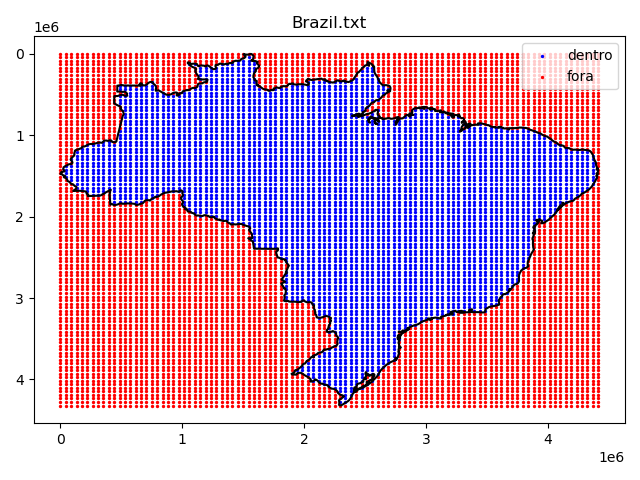
\includegraphics[width=1.0\textwidth]{figures/Brazil_grid.png}
        \end{overprint}
      \end{figure}
    \end{center}
    \column{0.33\textwidth}
    \begin{center}
      \begin{figure}
        \begin{overprint}
        \onslide<1>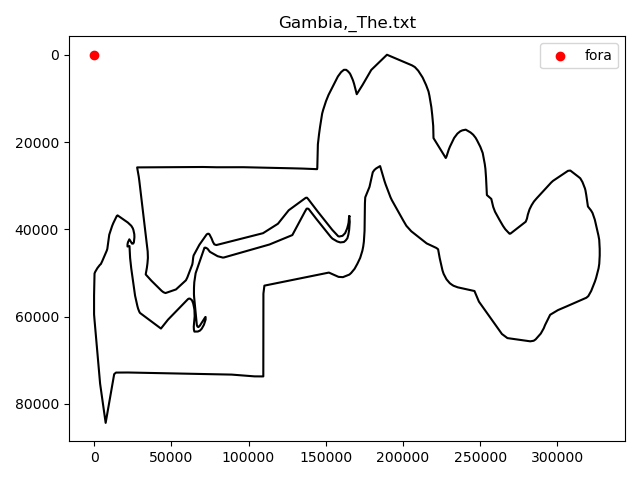
\includegraphics[width=1.0\textwidth]{figures/Gambia.png}
        \onslide<2>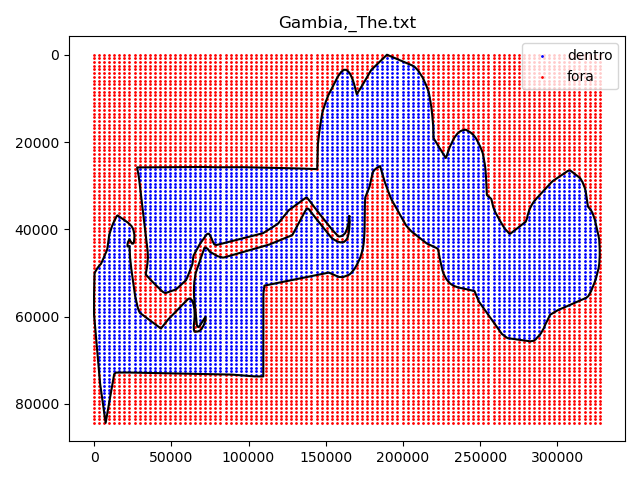
\includegraphics[width=1.0\textwidth]{figures/Gambia_grid.png}
        \end{overprint}
      \end{figure}
    \end{center}
  \end{columns}
\end{frame}

\begin{frame}{Polígonos Não-Simples}
  
  %add two columns
  \begin{columns}
    \column{0.5\textwidth}
    \begin{center}
      \begin{figure}
        \begin{overprint}
        \onslide<1>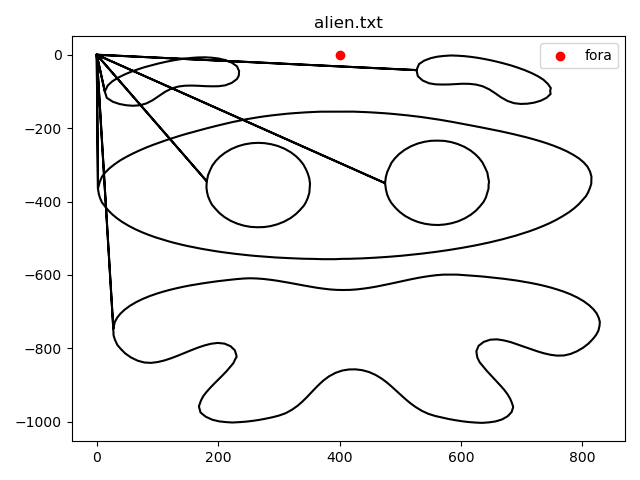
\includegraphics[width=1.0\textwidth]{figures/alien.png}
        \onslide<2>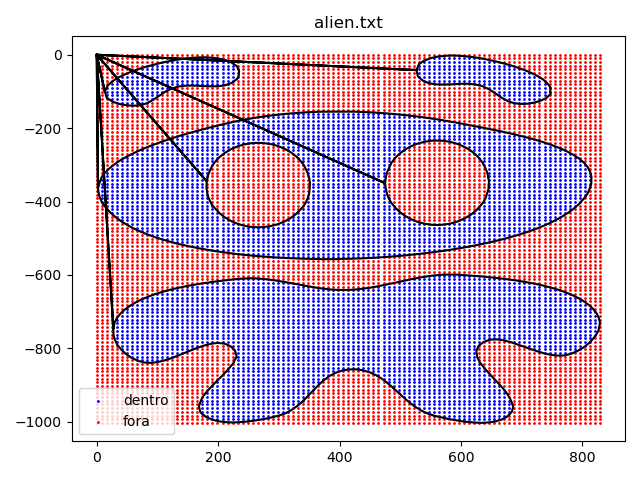
\includegraphics[width=1.0\textwidth]{figures/alien_grid.png}
        \end{overprint}
      \end{figure}
    \end{center}
    \column{0.5\textwidth}
    \begin{center}
      \begin{figure}
        \begin{overprint}
        \onslide<1>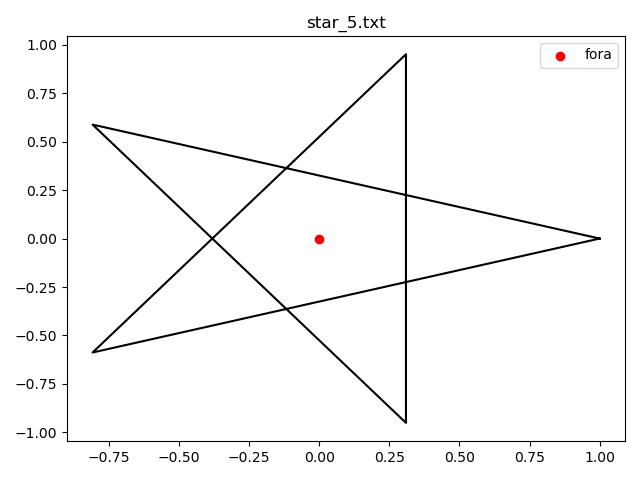
\includegraphics[width=1.0\textwidth]{figures/star_5.png}
        \onslide<2>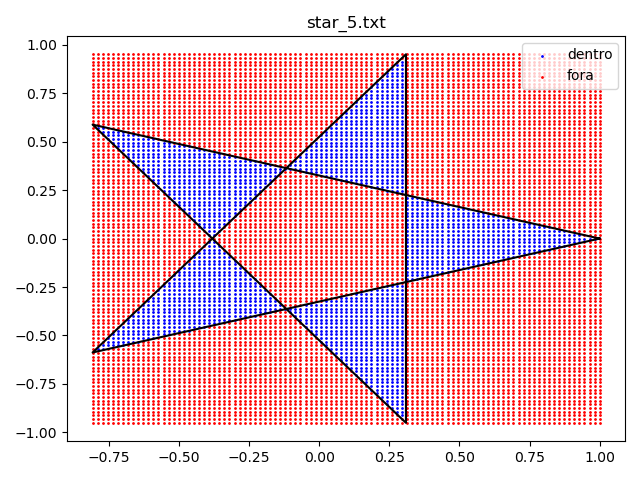
\includegraphics[width=1.0\textwidth]{figures/star_5_grid.png}
        \end{overprint}
      \end{figure}
    \end{center}
  \end{columns}

\end{frame}


\begin{frame}{Performance}

  \begin{columns}
    \column{0.5\textwidth}
    \begin{center}
      \begin{itemize}
        \item Execução com polígonos regulares
        \item Tamanhos de 10 a $10^7$ lados
        \item 5 execuções com cada tamanho
      \end{itemize}
    \end{center}
    \column{0.5\textwidth}
    \begin{center}   
      \begin{figure}
        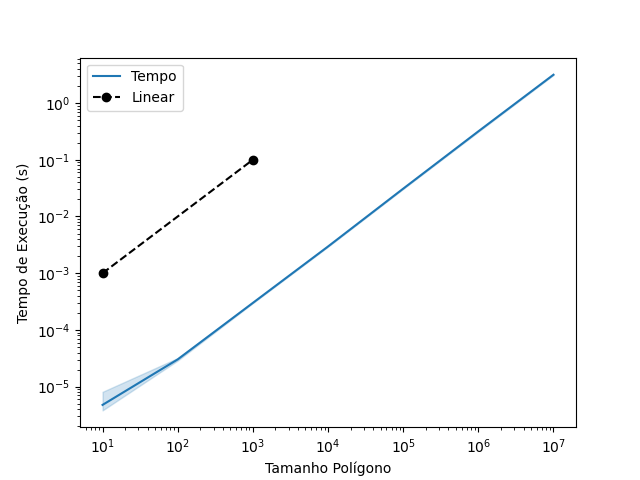
\includegraphics[width=1.0\textwidth]{figures/performance.png}
      \end{figure}
    \end{center}
  \end{columns}

\end{frame}

\begin{frame}
\frametitle{Conclusões}

\begin{itemize}
  \item O algoritmo funciona para polígonos simples
  \item O algoritmo tratou bem o caso das "quinas"
  \item O algoritmo tem resultado que é "razoável" no caso não-simples
  \item O tempo de execução é proporicional ao número de arestas
\end{itemize}

\end{frame}

\end{document}
